% 108-11~14(인쇄 108쪽) — 공통 지시문의 세 정규분포곡선 A, B, C(A 와 B 는 모양이 같고, B 와 C 는 대칭축이 같다 · 대칭축은 점선).
% 스캔 화질이 낮아 TikZ 로 다시 그림. 라벨은 원문에 있는 것만(A, B, C, x) · 대칭축의 값·대소 관계는 그림에 적지 않는다.
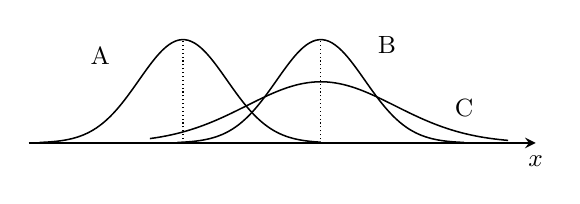
\begin{tikzpicture}[x=0.70cm, y=1.05cm, line width=0.55pt, font=\small]
  \draw[->, >=stealth, line width=0.7pt] (-4.3,0) -- (4.9,0) node[below=1pt] {$x$};
  \draw plot[domain=-4.1:1.0, samples=90, smooth] ({\x},{1.25*exp(-(\x+1.5)*(\x+1.5)/(2*0.80*0.80))});
  \draw plot[domain=-1.6:3.6, samples=90, smooth] ({\x},{1.25*exp(-(\x-1.0)*(\x-1.0)/(2*0.80*0.80))});
  \draw plot[domain=-2.1:4.4, samples=90, smooth] ({\x},{0.74*exp(-(\x-1.0)*(\x-1.0)/(2*1.35*1.35))});
  \draw[densely dotted, line width=0.4pt] (-1.5,0) -- (-1.5,1.25);
  \draw[densely dotted, line width=0.4pt] (1.0,0) -- (1.0,1.25);
  \node at (-3.0,1.05) {$\mathrm{A}$};
  \node at (2.2,1.18) {$\mathrm{B}$};
  \node at (3.6,0.42) {$\mathrm{C}$};
\end{tikzpicture}
